% !TeX program = pdfLaTeX
\documentclass[12pt]{article}
\usepackage{amsmath}
\usepackage{graphicx,psfrag,epsf}
\usepackage{enumerate}
\usepackage{natbib}
\usepackage{textcomp}
\usepackage[hyphens]{url} % not crucial - just used below for the URL
\usepackage{hyperref}

%\pdfminorversion=4
% NOTE: To produce blinded version, replace "0" with "1" below.
\newcommand{\blind}{0}

% DON'T change margins - should be 1 inch all around.
\addtolength{\oddsidemargin}{-.5in}%
\addtolength{\evensidemargin}{-.5in}%
\addtolength{\textwidth}{1in}%
\addtolength{\textheight}{1.3in}%
\addtolength{\topmargin}{-.8in}%

%% load any required packages here



% tightlist command for lists without linebreak
\providecommand{\tightlist}{%
  \setlength{\itemsep}{0pt}\setlength{\parskip}{0pt}}



\usepackage{float}
\usepackage{mathtools}
\usepackage{natbib}
\usepackage[linesnumbered,ruled,vlined]{algorithm2e}
\usepackage{verbatim}
\usepackage{amsthm}
\usepackage{comment}
\usepackage{amsfonts}

\begin{document}


\def\spacingset#1{\renewcommand{\baselinestretch}%
{#1}\small\normalsize} \spacingset{1}


%%%%%%%%%%%%%%%%%%%%%%%%%%%%%%%%%%%%%%%%%%%%%%%%%%%%%%%%%%%%%%%%%%%%%%%%%%%%%%

\if0\blind
{
  \title{\bf Manifold Clustering in the Generalized Random Dot Product
Graph}

  \author{
        John Koo \\
    Department of YYY, University of XXX\\
      }
  \maketitle
} \fi

\if1\blind
{
  \bigskip
  \bigskip
  \bigskip
  \begin{center}
    {\LARGE\bf Manifold Clustering in the Generalized Random Dot Product
Graph}
  \end{center}
  \medskip
} \fi

\bigskip
\begin{abstract}
The text of your abstract. 200 or fewer words.
\end{abstract}

\noindent%
{\it Keywords:} block models, community detection, coordinate descent,
latent structure models, manifold clustering, random dot product graph
\vfill

\newpage
\spacingset{1.45} % DON'T change the spacing!

\newcommand{\diag}{\mathrm{diag}}
\newcommand{\tr}{\mathrm{Tr}}
\newcommand{\blockdiag}{\mathrm{blockdiag}}
\newcommand{\indep}{\stackrel{\mathrm{ind}}{\sim}}
\newcommand{\iid}{\stackrel{\mathrm{iid}}{\sim}}
\newcommand{\Bernoulli}{\mathrm{Bernoulli}}
\newcommand{\Betadist}{\mathrm{Beta}}
\newcommand{\BG}{\mathrm{BernoulliGraph}}
\newcommand{\Uniform}{\mathrm{Uniform}}
\newcommand{\PABM}{\mathrm{PABM}}
\newcommand{\RDPG}{\mathrm{RDPG}}
\newcommand{\GRDPG}{\mathrm{GRDPG}}
\newcommand{\Multinomial}{\mathrm{Multinomial}}
\newtheorem{theorem}{Theorem}
\newtheorem{lemma}{Lemma}
\newtheorem{proposition}{Proposition}
\theoremstyle{remark}
\newtheorem{remark}{Remark}
\theoremstyle{definition}
\newtheorem{definition}{Definition}
\newtheorem{example}{Example}
\newcommand{\dd}{\mathrm{d}}
\newcommand{\as}{\stackrel{\mathrm{a.s.}}{\to}}
\newcommand{\ER}{\text{Erd\"{o}s-R\'{e}nyi}}

\hypertarget{introduction}{%
\section{Introduction}\label{introduction}}

We define a \emph{Bernoulli graph} as a random graph model for which
edge probabilities are contained in an edge probability matrix
\(P \in [0, 1]^{n \times n}\), and an edge occurs between vertices \(i\)
and \(j\) with probability \(P_{ij}\). Common random graph models then
impose structure on \(P\), based on various assumptions about the way in
which the data are generated, or to allow \(P\) to be estimated. One
example is the \(\text{Erd\"{o}s-R\'{e}nyi}\) model, in which all edge
probabilities are fixed, i.e., \(P_{ij} = p\).

One common analysis task for graph and network data is community
detection, which assumes that each vertex of a graph has a hidden
community label. The goal of the analysis is then to retrieve these
labels. In order to perform this analysis as a statistical inference
task is to define a probability model with inherent community structure.
We call such models \emph{block models}: First, each vertex is assigned
a label \(z_1, ..., z_n \in \{1, 2, ..., K\}\) where \(K \ll n\). Then
each edge probability \(P_{ij}\) is said to depend on the labels \(z_i\)
and \(z_j\), possibly along with some other parameters. For example, the
stochastic block model (SBM) sets a fixed edge probability for each pair
of communities, i.e., \(P_{ij} = \omega_{z_i, z_j}\). The
degree-corrected block model (DCBM) assigns an additional parameter
\(\theta_i\) to each vertex by which edge probabilities are scaled,
i.e., \(P_{ij} = \theta_i \theta_j \omega_{z_i, z_j}\). The popularity
adjusted block model (PABM) assigns \(K\) parameters to each vertex
\(\lambda_{i1}, \lambda_{i2}, ..., \lambda_{iK}\) that describe that
vertex's affinity toward each community; the edge probability between
vertices \(i\) and \(j\) is then defined as the product of vertex
\(i\)'s affinity toward vertex \(j\)'s community and vertex \(j\)'s
affinity toward vertex \(i\)'s community, i.e.,
\(P_{ij} = \lambda_{i z_j} \lambda_{j z_i}\).

The three block model types, as well as the
\(\text{Erd\"{o}s-R\'{e}nyi}\) model, impose structure on \(P\),
including on the rank of \(P\). \(P\) has rank 1 for the
\(\text{Erd\"{o}s-R\'{e}nyi}\) model, rank \(K\) for the SBM and DCBM,
and rank \(K^2\) for the PABM. This provides the intuition behind
another family of Bernoulli graphs called the \emph{random dot product
graph} (RDPG) and \emph{generalized random dot product graph} (GRDPG).
In the RDPG, each vertex has a corresponding latent vector in
\(d\)-dimensional Euclidean space, where \(d\) is the rank of \(P\) and
\(P\) is positive semidefinite. Then the edge probability between each
pair of vertices is defined as the inner product between the
corresponding latent vectors, i.e., \(P_{ij} = x_i^\top x_j\). If the
latent vectors are collected in a data matrix
\(X = \bigl[ x_1 \mid \cdots \mid x_n \bigr]^\top\), then the edge
probability matrix for the RDPG is \(P = X X^\top\). Similarly, the edge
probability between each pair of vertices for the GRDPG is defined as
the indefinite inner product between the corresponding latent vectors,
i.e., \(P_{ij} = x_i^\top I_{p,q} x_j\), where
\(I_{p,q} = \mathrm{blockdiag}(I_p, -I_q)\) and \(p + q = d\). Then the
edge probability matrix for the GRDPG is \(P = X I_{p,q} X^\top\). This
allows for a model similar to the RDPG for non-positive semidefinite
\(P\). While the RDPG and GRDPG do not necessarily have community
structure, it has been shown that block models are specific cases of the
RDPG or GRDPG in which latent vectors are organized by community. This
includes the SBM, in which communities correspond to point masses, DCBM,
in which communities correspond to line segments, and PABM, in which
communities correspond to orthogonal subspaces. In this work, we extend
this idea to communities organized into more general latent structures.
In particular, we assume that each community corresponds to a manifold
in the latent space.

\hypertarget{generalized-random-dot-product-graphs-with-community-structure}{%
\section{Generalized Random Dot Product Graphs with Community
Structure}\label{generalized-random-dot-product-graphs-with-community-structure}}

All Bernoulli graphs are generalized random dot product graphs. Whether
this is useful for inference depends on the structure of the latent
space. In the case of the \(\text{Erd\"{o}s-R\'{e}nyi}\) model, SBM,
DCBM, and PABM, the latent structure is linear, and the linearity can be
exploited for community detection and parameter estimation. In this
section, we discuss general, often nonlinear latent structure models,
focusing on those with community structure.

To motivate this, consider a generalization of the
\(\text{Erd\"{o}s-R\'{e}nyi}\) model. Recall that when viewed as an
RDPG, the latent space of an \(\text{Erd\"{o}s-R\'{e}nyi}\) model
consists of one point in Euclidean space. In the following example,
instead of fixing the edge probability, it is sampled from a
distribution in such a way that when viewed as an RDPG, the latent space
consists of a curve.

\begin{example}[Hierarchical $\text{Erd\"{o}s-R\'{e}nyi}$ model]
In the $\text{Erd\"{o}s-R\'{e}nyi}$ model, the edge probability matrix has a fixed value $[P_{ij}] \equiv p \in [0, 1]$. 
Suppose instead that each $P_{ij}$ is drawn from a distribution with density $f(p) = \frac{1}{\frac{\pi}{2} - 1} \Big(\frac{1}{\sqrt{1 - p^2}} - 1 \Big)$. 

Then it can be shown that this model is equivalent to a random dot product graph with a two dimensional latent space in which latent vectors are sampled uniformly along the curve $g(t) = \begin{bmatrix} \cos(\frac{\pi}{2} t) & \sin(\frac{\pi}{2} t) \end{bmatrix}^\top$, $0 \leq t \leq 1$. 
\end{example}

\begin{definition}[Manifold block model]
Let $p, q \geq 0$, $d = p + q \geq 1$, $K \geq 1$, and $n \geq 1$ be integers.
If there are manifolds $\mathcal{M}_1, ..., \mathcal{M}_K \subset \mathcal{X}$ for $\mathcal{X} = \{x, y \in \mathbb{R}^d : x^\top I_{p,q} y \in [0, 1] \}$, and 
$X = \begin{bmatrix} x_1 & \cdots & x_n \end{bmatrix}^\top$ such that each $x_i \in \mathcal{M}_k$ for some $k \in [K]$, then $A \sim \mathrm{GRDPG}_{p,q}(X; \rho_n)$ is a \emph{manifold block model}.
\end{definition}

In practice, we often define each manifold \(\mathcal{M}_k\) by a
continuous function \(g_k : [0, 1]^r \to \mathcal{X}\), where
\(1 \leq r < d\) is the dimensionality of manifold \(\mathcal{M}_k\). To
complete the probability model, we define a probability distribution
\(F\) with support \([0, 1]^r\) and draw the community memberships from
a multinomial distribution.

The full mixture model can be described as follows:

\begin{enumerate}
\def\labelenumi{\arabic{enumi}.}
\tightlist
\item
  Draw labels
  \(z_1, ..., z_n \stackrel{\mathrm{iid}}{\sim}\mathrm{Multinomial}(\alpha_1, ..., \alpha_K)\).
\item
  Draw latent vectors by first drawing each
  \(t_1, ..., t_n \stackrel{\mathrm{iid}}{\sim}F\) and then computing
  each \(x_i = g_{z_i}(t_i)\).
\item
  Let \(X = \begin{bmatrix} x_1 & \cdots & x_n \end{bmatrix}^\top\), and
  draw \(A \sim \mathrm{RDPG}(X)\) or
  \(A \sim \mathrm{GRDPG}_{p,q}(X)\).
\end{enumerate}

\begin{example}
Let $p = 2$, $q = 0$, $K = 2$, and $r = 1$. 
Define two one-dimensional manifolds by $f_1(t) = \begin{bmatrix} \cos(\frac{\pi}{3} t) & \sin(\frac{\pi}{3} t) \end{bmatrix}^\top$ and $f_2(t) = \begin{bmatrix} 1 - \cos(\frac{\pi}{3} t) & 1 - \sin(\frac{\pi}{3} t) \end{bmatrix}^\top$.
Draw $t_1, ..., t_n \stackrel{\mathrm{iid}}{\sim}\mathrm{Uniform}(0, 1)$ and $z_1, ..., z_n \stackrel{\mathrm{iid}}{\sim}\mathrm{Multinomial}(\frac{1}{2}, \frac{1}{2})$, and compute latent vectors $x_i = f_{z_i}(t_i)$, which are collected in data matrix $X = \begin{bmatrix} x_1 & \cdots & x_n \end{bmatrix}^\top$. 
Finally, let $A \sim \mathrm{RDPG}(X)$. Fig \ref{fig:example1} shows the latent configuration drawn from this latent distribution, a random dot product graph drawn from the latent configuration, and the adjacency spectral embedding of the graph. 

\begin{figure}[H]

{\centering 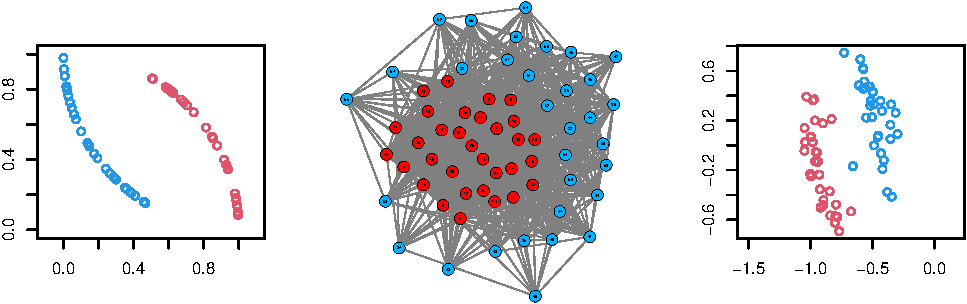
\includegraphics{draft_files/figure-latex/example1-1} 

}

\caption{Manifold block model described in Example 1. The latent configuration is on the left, and a random dot product graph drawn from the latent configuration is on the middle, and the ASE is on the right.}\label{fig:example1}
\end{figure}
\end{example}

\hypertarget{methods}{%
\section{Methods}\label{methods}}

We provide two approaches to community detection for the manifold block
model. First, we consider the case in which communities correspond to
manifolds in the latent space that do not intersect and are separated by
some finite distance. In this scenario, we use the convergence of the
ASE to show that single linkage clustering on the latent space produces
a clustering such that the total number of misclustered vertices goes to
zero, with high probability.

Next, we consider the case in which communities correspond to
one-dimensional manifolds in the latent space and may or may not
intersect. In this scenario, we propose an alternating coordinate
descent algorithm that alternates between estimating the structure of
the manifolds and the community labels, which we call \(K\)-curves
clustering. We again use the convergence of the ASE to show that under
certain conditions, \(K\)-curves clustering produces a clustering such
that the proportion of misclustered vertices goes to zero, with high
probability.

\hypertarget{nonintersecting-manifolds}{%
\subsection{Nonintersecting Manifolds}\label{nonintersecting-manifolds}}

\label{section:nonintersecting}

In this section, we consider the following scenario: Suppose that each
community is represented by a closed manifold \(\mathcal{M}_k\),
\(k \in \{1, ..., K\}\) in the latent space of a RDPG or GDRPG. Define
\(\delta = \min\limits_{k \neq \ell} \min\limits_{x \in \mathcal{M}_k, y \in \mathcal{M}_\ell} \|x - y\|\),
the minimum distance between two manifolds. We assume that
\(\delta > 0\), i.e., the manifolds do not intersect.

In the noiseless setting, if the subsample on each manifold is
sufficiently dense, it is possible to construct for each manifold an
\(\eta_k\)-neighborhood graph for each manifold for some \(\eta_k > 0\)
such that the graph is connected. Then if
\(\max_k \eta_k = \eta < \delta\), an \(\eta\)-neighborhood graph for
the entire sample will consist of \(K\) disconnected subgraphs that map
onto each manifold. Equivalently, we can apply single-linkage
clustering. The remainder of this section explores under which
conditions these criteria are met for the latent configuration, in which
latent vectors lie exactly on manifolds, as well as the ASE, which
introduces noise.

\begin{algorithm}[h]
\DontPrintSemicolon
\SetAlgoLined
\KwData{Adjacency matrix $A$, number of communities $K$, embedding dimensions $p$ and $q$.}
\KwResult{Community assignments $z_1, ..., z_n \in \{1, ..., K\}$.}
Compute $\hat{X}$, the ASE of $A$ using the $p$ most positive and $q$ most negative eigenvalues and their corresponding eigenvectors.\;
Apply single linkage clustering with $K$ communities on $\hat{X}$.\;
\caption{ASE clustering for nonintersecting communities.}
\end{algorithm}

Let \(F_k\) be a probability distribution with support
\(\mathcal{M}_k\). Then we define a mixture model as follows:

\begin{enumerate}
\def\labelenumi{\arabic{enumi}.}
\tightlist
\item
  Draw labels
  \(z_1, ..., z_n \stackrel{\mathrm{iid}}{\sim}\mathrm{Multinomial}(\alpha_1, ..., \alpha_K)\).
\item
  Draw latent vectors each as
  \(x_i \stackrel{\mathrm{ind}}{\sim}F_{z_i}\) for distributions
  \(F_1, ..., F_K\) with respective supports
  \(\mathcal{M}_1, ..., \mathcal{M}_K\).
\item
  Let \(X = \begin{bmatrix} x_1 & \cdots & x_n \end{bmatrix}^\top\), and
  draw \(A \sim \mathrm{RDPG}(X)\) or
  \(A \sim \mathrm{GRDPG}_{p,q}(X)\).
\end{enumerate}

Note that here, we redefine the model to ignore \(g_1, ..., g_K\), the
parameterizations of each manifold. Instead, we sample points directly
on the manifolds themselves. We will return to the parameterizations in
Section \ref{section:intersecting}.

\begin{theorem}[Community detection for nonintersecting manifolds without noise]
\label{nonintersect-no-noise}
Let $x_1, ..., x_n$ be points sampled on $K$ manifolds $\mathcal{M}_1, ..., \mathcal{M}_K$. 
Suppose $\delta = \min\limits_{k \neq \ell} \min\limits_{x_i \in \mathcal{M}_k, x_j \in \mathcal{M}_\ell} \| x_i - x_j \| > 0$. 
Define $A_n$ as the event that for a $\eta$-neighborhood graph constructed from the sample $x_1, ..., x_n$ consists of exactly $K$ disconnected subgraphs that map on exactly to each manifold for some $\eta \in (0, \delta)$. 
Then for any $\epsilon \in (0, 1)$, there exists an $N$ such that when $n > N$, $A_n$ occurs with high probability. 
\label{nonintersect-no-noise}
\end{theorem}

\hypertarget{intersecting-manifolds}{%
\subsection{Intersecting Manifolds}\label{intersecting-manifolds}}

\label{section:intersecting}

In this section, we again consider the setting for the RDPG or GRDPG in
which each community lies on a manifold in the latent space. However,
this time, we do not assume that the manifolds are nonintersecting. We
also restrict this case to one-dimensional manifolds which are each
described by \(g_k : [0, 1] \to \mathcal{X}\). Then we define a mixture
model as follows:

\begin{enumerate}
\def\labelenumi{\arabic{enumi}.}
\tightlist
\item
  Draw \(t_1, ..., t_n \stackrel{\mathrm{iid}}{\sim}F\) for probability
  distribution \(F\) with support \([0, 1]\).
\item
  Draw
  \(z_1, ..., z_n \stackrel{\mathrm{iid}}{\sim}\mathrm{Multinomial}(\alpha_1, ..., \alpha_K)\),
  the community labels.
\item
  Let each \(x_i = g_{z_i}(t_i)\) be the latent vector for vertex
  \(v_i\), and collect the latent vectors into matrix
  \(X = \begin{bmatrix} x_1 & \cdots & x_n \end{bmatrix}^\top\).
\item
  Draw \(A \sim \mathrm{RDPG}(X)\) or
  \(A \sim \mathrm{GRDPG}_{p,q}(X)\).
\end{enumerate}

\begin{algorithm}[h]
\DontPrintSemicolon
\SetAlgoLined
\KwData{Adjacency matrix $A$, number of communities $K$, embedding dimensions $p$, $q$, stopping criterion $\epsilon$}
\KwResult{Community assignments $1, ..., K$, curves $g_1, ..., g_K$}
Compute $X$, the ASE of $A$ using the $p$ most positive and $q$ most negative eigenvalues and their corresponding eigenvectors.\;
Initialize community labels $z_1, ..., z_n$.\;
\Repeat {the change in $\sum_k \sum_{i \in C_k} \|x_i - g_k(t_i)\|^2$ is less than $\epsilon$} {
\For {$k = 1, ..., K$} {
Define $X_k$ as the rows of $X$ for which $z_i = k$.\;
Fit curve $g_k$ and positions $t_{k_i}$ to $X_k$ by minimizing $\sum_{k_i} \|x_{k_i} - g_k(t_{k_i})\|^2$.\;
}
\For {$k = 1, ..., K$} {
Assign $z_i \leftarrow \arg\min_\ell \|x_i - g_\ell(t_i)\|^2$.\
}
}
\caption{$K$-curves clustering.}
\end{algorithm}

\begin{theorem}
\label{k-curves-clustering}
Let each $g_k$ be smooth. 
Then $K$-curves clustering converges to a stationary point of the objective, 
$\sum_k \sum_{i \in C_k} \|x_i - g_k(t_i)\|^2$.
\end{theorem}

\begin{proof}
$K$-curves clustering is a batch coordinate descent algorithm. 
Thus, in order to show that it converges to a stationary point, it is sufficient to show that each descent step decreases the objective function. 
\end{proof}

\(K\)-curves clustering assumes that the functional form of \(g_k\) is
known. The choice of \(g_k\) affects the difficulty of the algorithm. As
a balance between flexibility and ease of estimation, we consider the
case where each \(g_k\) is a Bezier polynomial of degree \(R\) with
coefficients \(p_k\). Then we have
\(g_k(t) = g(t; p_k) = \sum_{r=0}^R p_k^{(r)} \binom{R}{r} (1-t)^{R-r} t^r\).

Given \(\{t_i\}\) and \(\{z_i\}\), it is straightforward to obtain
\(\hat{p}_k = \arg\min_p \sum_{k_i} \|x_{k_i} - g_k (t_{k_i}; p)\|^2\)
\[\hat{p}_k = (T_k^\top T_k)^{-1} T_k^\top X_k,\] where \(T_k\) is an
\(n_k \times (R+1)\) matrix with rows
\(\begin{bmatrix} (1 - t_{k_i})^R & (1 - t_{k_i})^{R-1} t_{k_i} & \cdots & (1 - t_{k_i}) t_{k_i}^{R-1} & t_{k_i}^R \end{bmatrix}\).
Estimation of \(\{t_i\}\) given \(\{z_i\}\) and \(\{p_k\}\) is more
difficult. Each \(t_i\) can be estimated separately:
\begin{equation} \label{eq:min-t}
\hat{t}_i = \arg\min_t \|x_i - g(t; p_{z_i})\|^2. 
\end{equation} This is equivalent to solving
\(0 = (x_i - g(t; p_{z_i}))^\top (\dot{g}(t; p_{z_i}))\). Setting
\(c^{(s)} = \sum_{r=0}^s (-1)^{s-r} \binom{R}{r} p^{(r)}_{z_i}\) for
\(s \neq 0\) and \(c^{(0)} = p^{(0)}_{z_i} - x_i\), let
\(c = \begin{bmatrix} c^{(0)} & \cdots & c^{(R)} \end{bmatrix}^\top\).
Then solving Eq. \ref{eq:min-t} is equivalent to finding the real roots
of a polynomial with coefficients that are the sums of the reverse
diagonals of \(C D^\top\), where \(C_{ij} = c_{ij} (-1)^i \binom{R}{i}\)
and \(D_{ij} = c_{i-1,j} (-1)^{i-1} \binom{R-1}{i-1}\).

\begin{algorithm}[h]
\DontPrintSemicolon
\SetAlgoLined
\KwData{Adjacency matrix $A$, number of communities $K$, embedding dimensions $p$, $q$, stopping criterion $\epsilon$, $m_k \leq n_k$ known community assignments for each community}
\KwResult{Community assignments $1, ..., K$, curves $g_1, ..., g_K$}
Compute $X$, the ASE of $A$ using the $p$ most positive and $q$ most negative eigenvalues and their corresponding eigenvectors.\;
Fit curves $g_1, ..., g_K$ using each of the $m_1, ..., m_K$ points with known community labels by minimizing $\sum_{j=1}^{m_i} \|x_j - g_k(t_j)\|^2$.\;
Assign labels $z_1, ..., z_n$ to each $x_1, ..., x_n$ by minimizing $\|x_i - g_k(t_i)\|^2$ for $k$, holding the initial known labels constant.\; 
\Repeat {the change in $\sum_k \sum_{i \in C_k} \|x_i - g_k(t_i)\|^2$ is less than $\epsilon$} {
\For {$k = 1, ..., K$} {
Define $X_k$ as the rows of $X$ for which $z_i = k$.\;
Fit curve $g_k$ and positions $t_{k_i}$ to $X_k$ by minimizing $\sum_{k_i} \|x_{k_i} - g_k(t_{k_i})\|^2$.\;
}
\For {$k = 1, ..., K$} {
Assign $z_i \leftarrow \arg\min_\ell \|x_i - g_\ell(t_i)\|^2$, holding the known initial labels constant.\
}
}
\caption{Semi-supervised $K$-curves clustering.}
\end{algorithm}

\begin{theorem}
Let each $g(\cdot; p_k)$ be a nonintersecting Bezier polynomial of order $R$, 
and a GRDPG is drawn from vectors that lie on the curves. 
Suppose we observe the true labels of $m_k$ vertices from each community, and each $m_k > R + 1$. Suppose further that latent vectors $x_j = g(t_i; p_{z_j})$ that correspond to vertices with observed labels are such that 
Then as $n \to \infty$, the proportion of misclustered vertices from $K$-curves clustering approaches $0$ with probability $1$.
\end{theorem}

\hypertarget{examples}{%
\section{Examples}\label{examples}}

\begin{example}
Here, $K = 2$ with $g_1(t) = \begin{bmatrix} t^2 & 2 t (1 - t) \end{bmatrix}^\top$ and $g_2(t) = \begin{bmatrix} 2 t (1 - t) & (1 - t) ^ 2 \end{bmatrix}^\top$. We draw $n_1 = n_2 = 2^8$ points uniformly from each curve. 

\begin{figure}[H]

{\centering 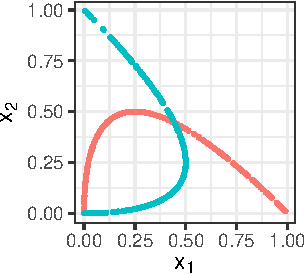
\includegraphics{draft_files/figure-latex/unnamed-chunk-2-1} 

}

\caption{Latent positions, labeled by curve/community.}\label{fig:unnamed-chunk-2}
\end{figure}

We draw $A \sim \mathrm{RDPG}(X)$ and obtain the following ASE:

\begin{figure}[H]

{\centering 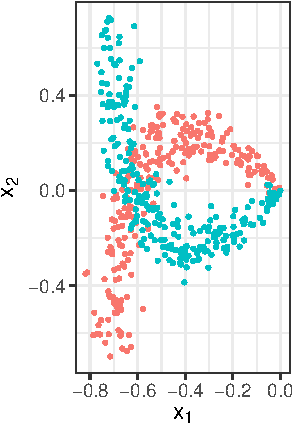
\includegraphics{draft_files/figure-latex/unnamed-chunk-3-1} 

}

\caption{ASE of an RDPG drawn from the latent positions, labeled by curve/community.}\label{fig:unnamed-chunk-3}
\end{figure}

We then try applying $K$-curves clustering to this graph. 
The first three are with random initial labels, forcing the intercept to be zero. 
The fourth initializes the labels randomly but allows the intercept to be nonzero. 
The fifth initializes the labels by spectral clustering with the normalized Laplacian, again forcing the intercept to be zero. 
The sixth also initializes via spectral clustering but allows the intercept to be nonzero. 





\begin{figure}[H]

{\centering 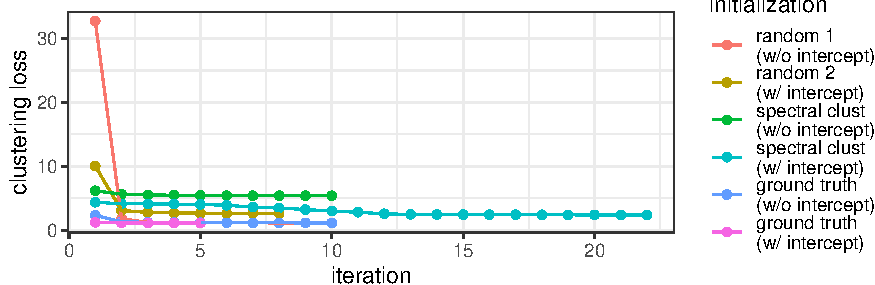
\includegraphics{draft_files/figure-latex/unnamed-chunk-6-1} 

}

\caption{Clustering loss vs. iteration for each run of K-curve clustering.}\label{fig:unnamed-chunk-6}
\end{figure}

\begin{figure}[H]

{\centering 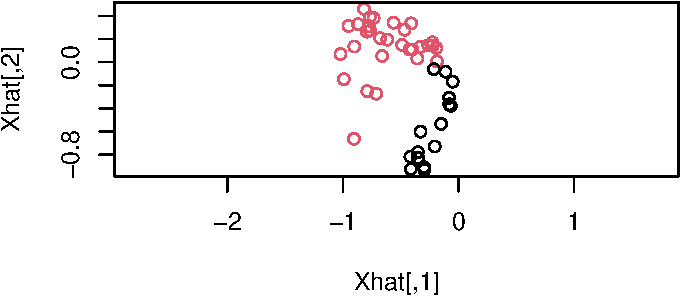
\includegraphics{draft_files/figure-latex/unnamed-chunk-7-1} 

}

\caption{ASE labeled by estimated community labels for each initialization strategy.}\label{fig:unnamed-chunk-7}
\end{figure}

\end{example}

\begin{example}[Macaque visuotactile brain areas and connections \citep{https://doi.org/10.1111/j.1460-9568.2006.04678.x}]


\begin{center}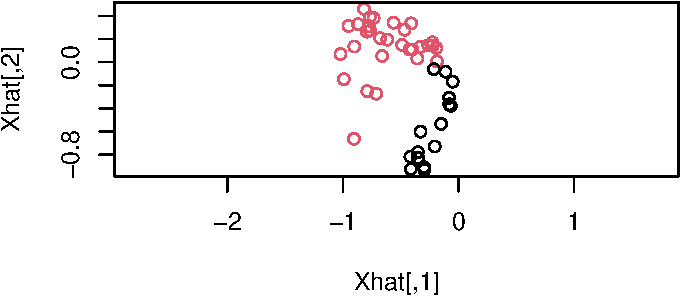
\includegraphics{draft_files/figure-latex/unnamed-chunk-8-1} \end{center}




\begin{center}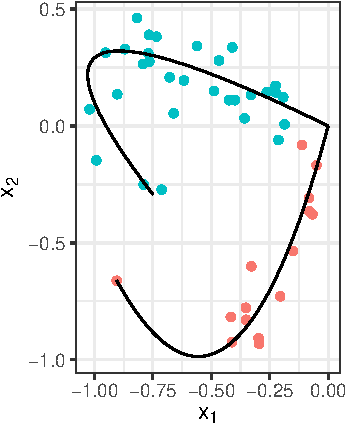
\includegraphics{draft_files/figure-latex/unnamed-chunk-10-1} \end{center}


\begin{center}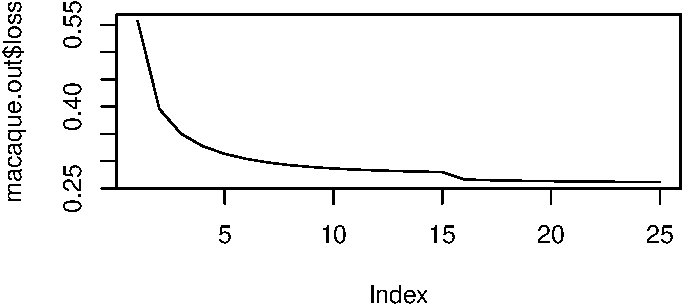
\includegraphics{draft_files/figure-latex/unnamed-chunk-11-1} \end{center}

\end{example}

\begin{example}[Non-intersecting curves]


\begin{center}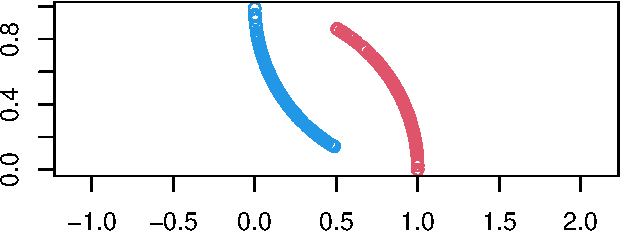
\includegraphics{draft_files/figure-latex/unnamed-chunk-12-1} \end{center}






\begin{center}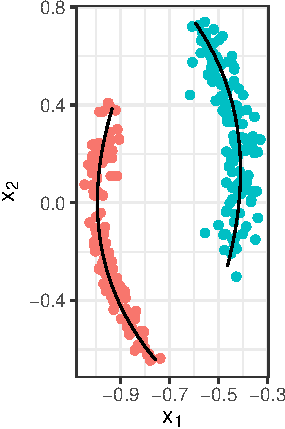
\includegraphics{draft_files/figure-latex/unnamed-chunk-15-1} \end{center}

\end{example}

\hypertarget{simulation-study}{%
\section{Simulation Study}\label{simulation-study}}

\hypertarget{discussion}{%
\section{Discussion}\label{discussion}}

\appendix

\section{Proofs of Theorems}

In order to prove theorem \ref{nonintersect-no-noise}, we first
establish that the density of points within one manifold is sufficiently
dense. The following lemma is based on lemma 2 of
\citet{trosset2020rehabilitating}.

\begin{lemma}
\label{lem:one-hypercube}
Let $x_1, ..., x_n \stackrel{\mathrm{iid}}{\sim}F$ with support $[0, 1]^r$, and $f(x) \geq a > 0$ everywhere on the support. 
Define $H_n$ as the event that an $\eta$-neighborhood graph constructed from the sample is connected for any $\eta > 0$. 
Then for any $\epsilon > 0$, there exists $N = O \bigg( \frac{\log \epsilon + r \log \eta - \frac{r}{2} \log r}{\log (1 - a \eta^r r^{-r / 2})} \bigg)$ such that $P(E_n) > 1 - \epsilon$ when $n \geq N$.
\end{lemma}

\begin{proof}
Divide the hypercube $[0, 1]^r$ into a grid of sub-hypercubes of side length at most $\eta / \sqrt{r}$. 
$E_n$ is satisfied if each sub-hypercube contains at least one $X_i$ from the sample. 

$$
\begin{aligned}
P(H_n) & = 1 - P(\text{some cells don't contain } X_i) \\
& \geq 1 - \sum_m^{\lceil \sqrt{r} / \eta \rceil^r} \prod_i^n P(X_i \text{ is not in the } k^{th} \text{ hypercube}) \\
& \geq 1 - \lceil \sqrt{r} / \eta \rceil^r (1 - a \eta^r / r^{r/2})^n,
\end{aligned}
$$
which approaches $1$ as $n \to \infty$. 
Setting this quantity as  $\geq 1 - \epsilon$ and solving for $n$ yields the desired rate. 
\end{proof}

\begin{lemma}
\label{lem:K-hypercubes}
Let there be $K \geq 2$ hypercubes $\mathcal{C}_1, ..., \mathcal{C}_K$ of dimension $r_1, ..., r_K$ in $\mathbb{R}^d$ such that $\delta = \min\limits_{k \neq \ell} \min\limits_{x_i \in \mathcal{C}_k, x_j \in \mathcal{C}_\ell} \|x_i - x_j\| > 0$. 
Let $F_k$ be a distribution with support $C_k$ such that its density $f_k$ is nonzero on the support. Let $a = \min_k \min_t f_k(t) > 0$. 
Define a mixture model as follows: 

\begin{enumerate}
  \item Draw labels $z_1, ..., z_n \stackrel{\mathrm{iid}}{\sim}\mathrm{Multinomial}(\alpha_1, ..., \alpha_K)$. 
  \item Draw latent vectors each as $x_i \stackrel{\mathrm{ind}}{\sim}F_{z_i}$.
\end{enumerate}

Define $H'_n$ as the event that an $\eta$-neighborhood graph constructed from this sample consists of exactly $K$ disconnected subgraphs for any $\eta \in (0, \delta)$. 
Then for any $\epsilon \in (0, 1)$, there exists an $N = O \Big( \frac{\log(1 - (1 - \epsilon)^{1/K}) + d \log \eta - \frac{d}{2} \log d}{\alpha_{min} \log(1 - a \eta^d d^{-d/2})} \Big)$ such that when $n > N$, $P(E_n) > 1 - \epsilon$. 
\end{lemma}

\begin{proof}
Let $H^{(k)}$ be the event that lemma \ref{lem:one-hypercube} holds for $\mathcal{C}_k$. Then $H^{(k)} = H_{n_k}$ where $H_n$ is defined as in \ref{lem:one-hypercube}. 
Then $P(H'_n) = P(H_{n_1} \text{ and } ... \text{ and } H_{n_K})$. 

$$
\begin{aligned}
P(H'_n) & = \prod_k P(H_{n_k}) \\
& \geq \prod_k 1 - \lceil \sqrt{r_k} / \eta \rceil^{r_k} (1 - a \eta^{r_k} r_k^{-r_k/2})^{n_k} \\
& \geq \prod_k 1 - \lceil \sqrt{d} / \eta \rceil^{d} (1 - a \eta^{d} d^{-d/2})^{\alpha_{\min} n} \\
& \geq \big(1 - \lceil \sqrt{d} / \eta \rceil^{d} (1 - a \eta^{d} d^{-d/2})^{\alpha_{\min} n} \big)^K, \\
\end{aligned}
$$
which approaches 1 as $n \to \infty$. 
Setting this quantity to $\geq 1 - \epsilon$ and solving for $n$ yields the desired rate. 
\end{proof}

\begin{proof}[Proof of theorem \ref{nonintersect-no-noise}]
\end{proof}

\section{Details on Fitting Bezier Curves with Noise}

\bibliographystyle{agsm}
\bibliography{bibliography.bib}


\end{document}
